\documentclass{article}
\usepackage{amsmath}
\usepackage{graphicx}
\title{Midterm Exam: Operating Systems}
\author{Quin'darius Lyles-Woods}
\begin{document}
\maketitle

\section{How does the kernel know if an application is in an infinite loop?}
It can tell through the kernel and its interrupt driven hardware and software. It will catch it through an exception or trap.
\section{Linux file has three levels of security associated with it that matches the three classes of users that may access that file. What are those?}

\begin{itemize}
	\item Owner
	\begin{itemize}
		\item Read
		\item Write
		\item Execute
	\end{itemize}
	\item Group
	\begin{itemize}
		\item Read
		\item Write
		\item Execute
	\end{itemize}
	\item Other
	\begin{itemize}
		\item Read
		\item Write
		\item Execute
	\end{itemize}
\end{itemize}

\section{All computers follow roughly the same set of steps to transition from a power-off state to a running state. Can you enumerate the steps of the booting sequence?}
\begin{verbatim}
                           +----------------------+                                      
                           |                      |                                      
                           |                      |                                      
+----------------------+   |                      |                                      
|o o o                 |   |  Loading the Kernel  |           Running                    
+----------------------+   |     Into Memory      |------------Kernel-----+              
|                      |   |                      |                       |              
|                      |   |                      |                       |              
|    Power is Off      |   |                      |                       v              
|                      |   +----------------------+         +---------------------------+
|                      |               ^                    |                           |
|                      |               |                    |                           |
+----------------------+           Locates                  |   System Boot Complete    |
            |                       Kernel                  |                           |
            |                          |                    |                           |
            |                          |                    |                           |
            |                          |                    +---------------------------+
            |                          |                                                 
            |            +--------------------------+                                    
        Power On         |                          |                                    
            |            |                          |                                    
            |            |  Fixed Memory Location   |                                    
            |            |      That Contains:      |                                    
            +----------->|        Bootloader        |                                    
                         |           BIOS           |                                    
                         |                          |                                    
                         |                          |                                    
                         |                          |                                    
                         +--------------------------+                                    
\end{verbatim}
\pagebreak
\section{Output redirection in Linux/UNIX system. We use \(>\) as well as \(>>\) as the output direction. What is the semantic difference between the two option switches?}
You take the output of a program and write it to a file the manner in which is done is discussed below.
\begin{itemize}
	\item [\(>\)] This is used for writing to a file and if the file already exist it will overwrite it.
	\item [\(>>\)] This is used for writing to a file and if the file already exist it will append to the file.
\end{itemize}
\section{What does the command \texttt{chmod 765 foo} tell the computer to do?}
Chmod is a program that defines the permissions of files and directories. 
\begin{itemize}
	\item [7: Owner] Read Write and Execute
	\item [6: Group] Read and Write
	\item [5: Other] Read Only
\end{itemize}
So the command means that the owner has full access, group only read and write and the others group only read only.
\section{What do you mean by big-endian and little-endian system?}
\begin{itemize}
	\item [Little Endian System] least significant value in the sequence is stored first in the computers memory.
	\item [Big Endian System] most significant value in the sequence is stored first in the computers memory.
\end{itemize}
\section{Keeping in mind the various definitions of \textbf{operating system}, consider whether the operating system should include applications such as web browsers and mail programs. Argue both that it should and that it should not, and support your answers.}
\subsection*{Should}
The operating system should handle the processes that are necessary for computing within the modern era. Currently the operating system only supports basic I/O within the computer but time has passed and its time for the operating system to start taking on more responsibility with tools that are now essential to modern computing. The OS needs to extend the basic I/O and expand the communications sector of the operating system to make sure these now commonplace tools are secure, stable and performant. 
\subsection*{Should Not}
The operating system is already a complex piece of software and the addition of other applications such as mail and browsers will be a redundancy on the core of what the operating system is already doing. There is a separation of abstraction that must be maintained or then the rules to what qualify as a essential operating system application will be twisted into all OS becoming bloated with unused applications. So one must take care to keep the operating system clean and minimal. 
\section{Explain the difference between a batch processing and multiprogramming.}
\begin{itemize}
	\item [Batch Processing] Grouping processes to be executed on after another. This is slower.
	\item [Multi Programming] Ability for the Operating System to perform multiple process on a single processor. This is faster.
\end{itemize}
\section{What is the purpose of the UNIX pipe command, i.e., vertical bar character \(|\)}
The purpose of piping is to send the output of one program to another so that it can be be executed as input to another program.
\section{Which of the following scheduling algorithms could result in starvation?}
\begin{itemize}
	\item [SJF] For long processes could never be executed and could lead to starvation if short jobs are continuously added.
	\item [Priority] If a process without a high prioity is in and there are task with slightly higher priority being added continously then the low priority will never be executed.
\end{itemize}
\section{What do you know about BIOS? In the class we discussed that PC/BIOS PROM monitor is rather limited in its ability to access the system hardware. What new standard is being proposed to replace the traditional legacy BIOS?}
The BIOS is what is used to locate the operating system and load the approiate software to make it work. Also has some basic low level drivers to allow someone to work with the computer via hardware inputs. The Unified Extensible Firmware Interface UEFI is slated to overtake the Basic Input Output System. 
\section{What is the purpose of interrupts? What are the differences between a trap and an interrupt? What is the use of each function? How are multiple interrupts dealt with? Can traps be generated intentionally by a user program? If so, for what purpose?}
The purpose of interrrupts is to stop the execution of the CPU. A trap is a software generated interrupt an interrupt is usally through memory or hardware like the keyboard or the mouse. You can use an interrupt when the processes isnt going as planned and you want to stop the process. Traps can be used to debug code. Multiple interrupts from traps are dealth with synchronously and asyncronously with IO interrupts. As explained early traps and be generated by the user for debugging purposes in softeware. 
\section{What is the purpose of system calls, and how do system calls relate to the OS and to the concept of dual-mode (kernel mode and user mode) operation?}
The purpose of system calls is to allow the user to make request to the operating system. System calls relate to the OS by using them to interface with the operating system and this is done within the context of user mode and group mode by explaining that when the user is logged in they are in "user mode" and when they use an application to make a system call the application takes advantage of the kernel mode and executes the task that was given to the computer from user mode. This is the concept of dual mode because you have 2 modes that you can operate within.
\section{Why do some operating systems store the operating system in firmware, while others store it on disk?}
Depends on the device, if the device has a disk drive than it is possible but if it is easier to store it on the computers memory that will make things simpler for that specific hardware. 
\section{Label the figure}
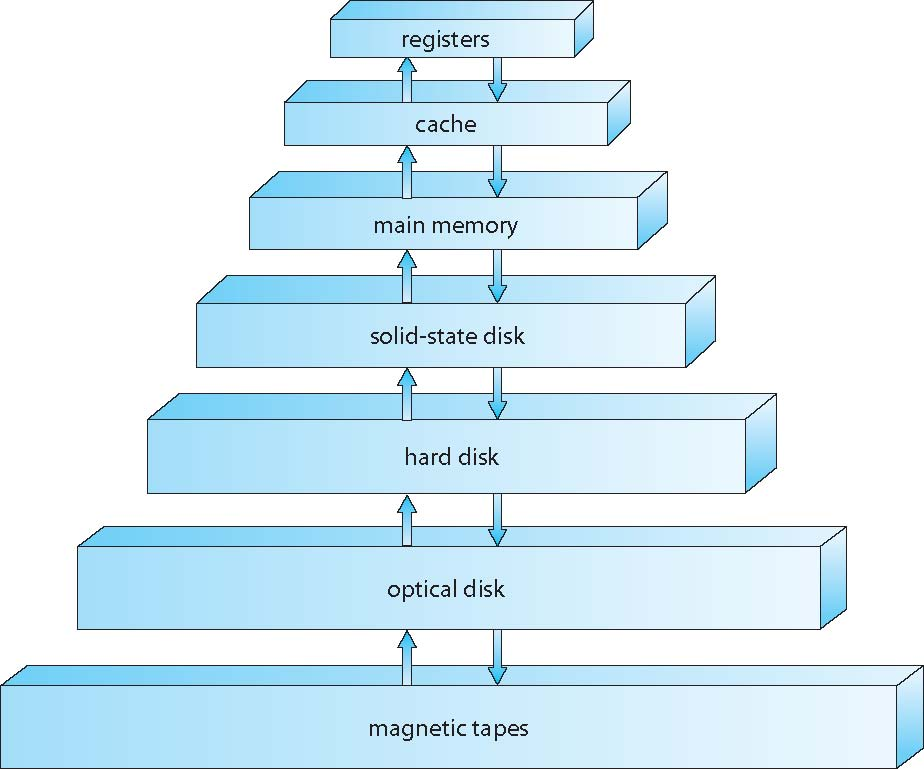
\includegraphics{memory}
\begin{itemize}
	\item[Registers]
		\begin{itemize}
			\item Primary
			\item Faster
			\item Smaller
			\item Volatile 
		\end{itemize}
	\item[Cache]
		\begin{itemize}
			\item Primary
			\item Faster
			\item Smaller
			\item Volatile 
		\end{itemize}
	\item[Main Memory]
		\begin{itemize}
			\item Primary
			\item Faster
			\item Large
			\item Volatile 
		\end{itemize}
	\item[Solid State Disk]
		\begin{itemize}
			\item Secondary 
			\item Faster
			\item Large
			\item Non-Volatile
		\end{itemize}
	\item[Hard Disk]
		\begin{itemize}
			\item Secondary 
			\item Faster
			\item Large
			\item Non-Volatile
		\end{itemize}
	\item[Optical Disk]
		\begin{itemize}
			\item Tertiary 
			\item Slower
			\item Large
			\item Non-Volatile
		\end{itemize}
	\item[Magnetic Tape]
		\begin{itemize}
			\item Tertiary 
			\item Slower
			\item Large
			\item Non-Volatile
		\end{itemize}
\end{itemize}
\section{Explain the figure. What is the role of the linker and the loader?}
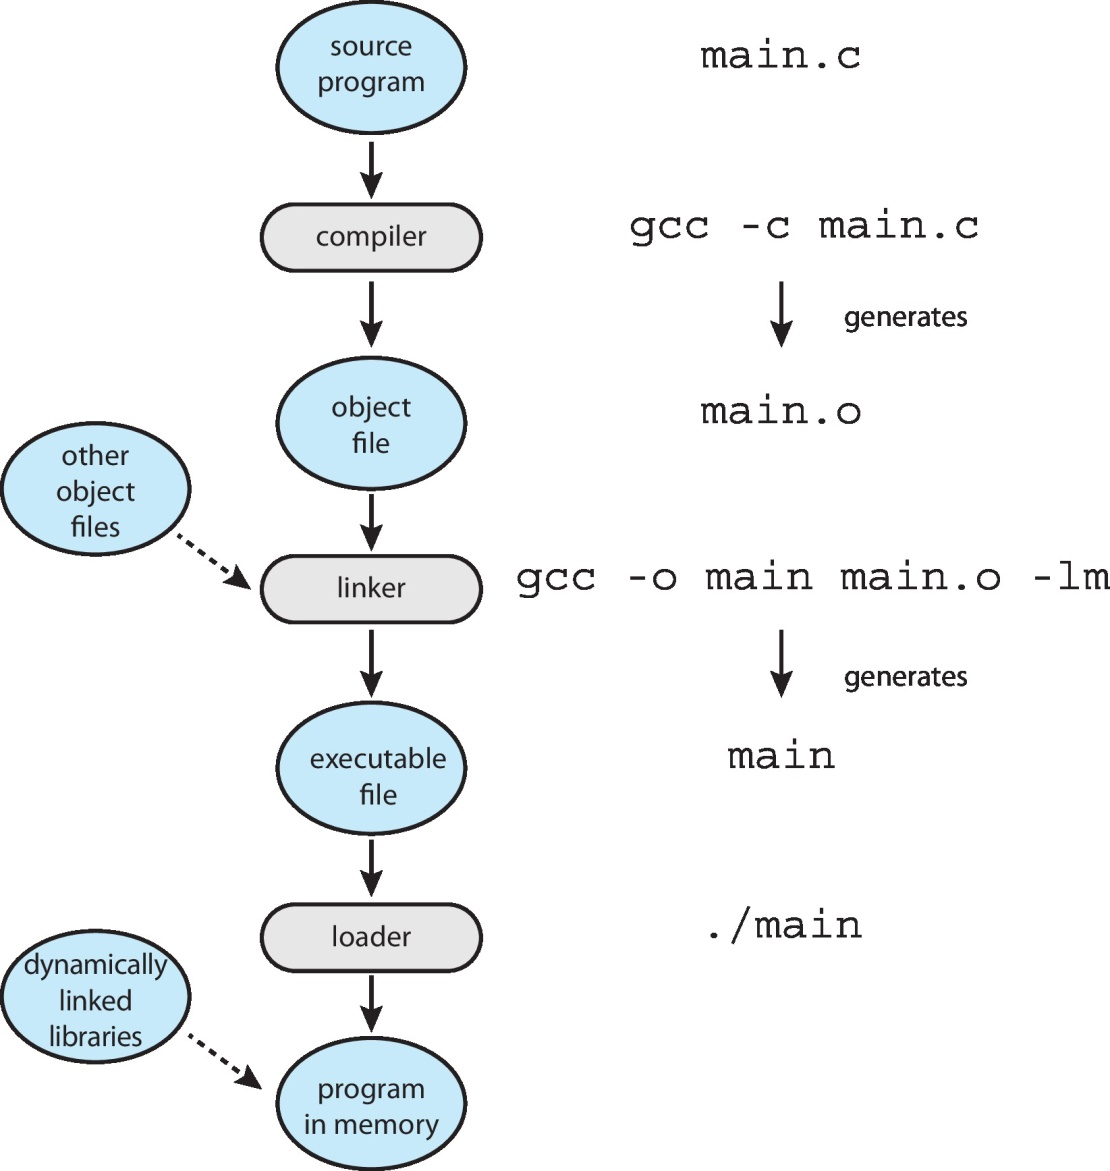
\includegraphics{linker_and_loader}
\begin{itemize}
	\item [Linker] The linker connects all the other files that are being used in the program, like STD Libraries and any thing that we have declared ourselves. This allows our program to be executable.
	\item [Loader] The loader moves the complied program from whatever kind of hard drive you are using to the main memory for you to execute. 
\end{itemize}
\section{Explain different parts of the memory and what is the purpose of those memory.}
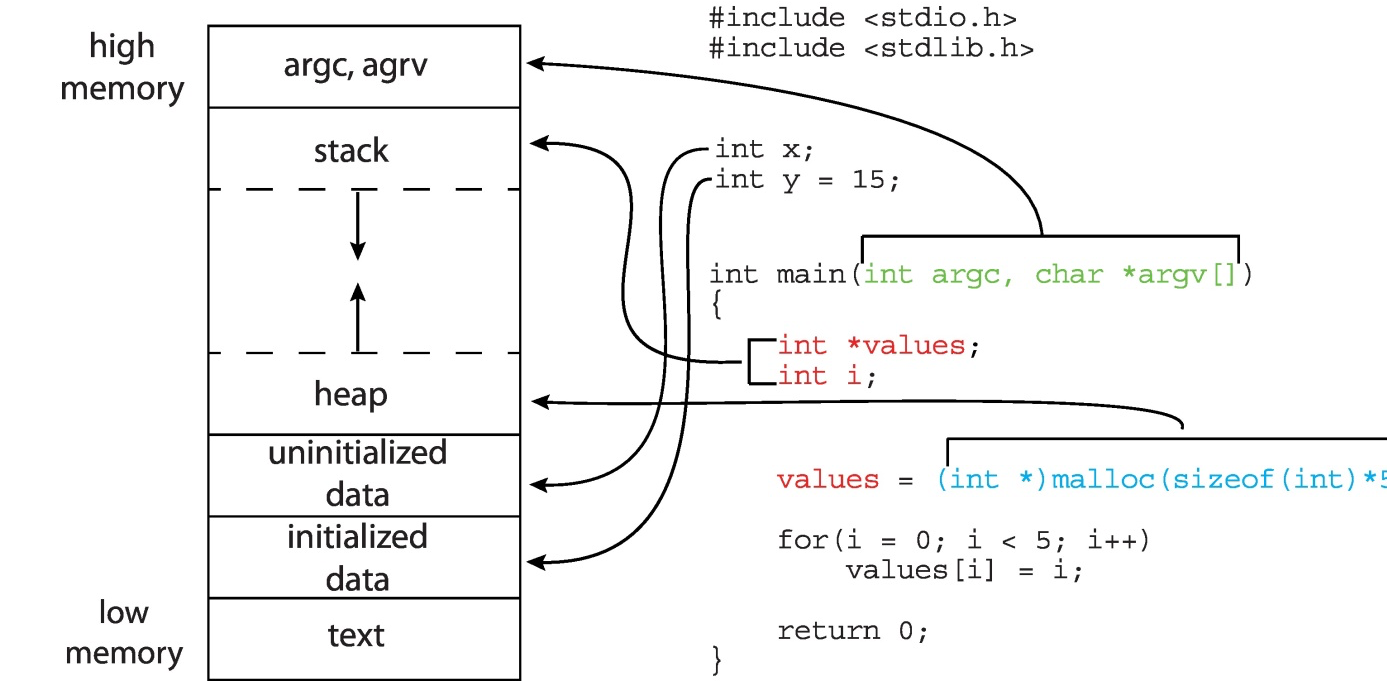
\includegraphics{program_memory}
\begin{itemize}
	\item [Arguments] Stores the amount of command line arguments passed to the program. 
	\item [Stack] Stores the local variables.
	\item [Heap] Stores the dynamic data structures. 
	\item [Initialized Data] Stored data that hasn't been initialized and that is not apart of the main program so not stored in the stack. 
	\item [Uninitialized Data] Stored data that has been initialized and that is part of the main program so not stored in the stack. 
	\item [Text]
\end{itemize}
\pagebreak
\section{Using Amdalh’s Law, calculate the speedup gain of an application that has 60 percent parallel component for (a) two processing cores and (b) four processing cores.}
\begin{center}
Review of the law
\end{center}
\[Speed\;Increase \le \frac{1}{Serial\;Portion+\frac{(1-Serial\;Portion)}{Cores}}\]
\[1.42 \le \frac{1}{.40+\frac{(1-.40)}{2}}\]
\[1.82 \le \frac{1}{.40+\frac{(1-.40)}{4}}\]
\end{document}
